\documentclass[11pt,a4paper]{article}

%\usepackage[utf8]{inputenc}
\usepackage{indentfirst}
\usepackage[hidelinks]{hyperref}
\usepackage{float}
\usepackage{array}
\usepackage{listings}
\usepackage{csquotes}
\usepackage{enumitem, amsmath, amssymb, amsfonts, latexsym, mathrsfs}
\usepackage{graphicx}
\usepackage{subfig}
%\usepackage[greek,english]{babel}
%\usepackage{alphabeta}
\usepackage{multicol}
\usepackage{bookmark}
\usepackage{caption}


% Setup de hiperenlaces
\hypersetup{
    colorlinks=true,
    linkcolor=cyan,
    filecolor=magenta,      
    urlcolor=cyan,
    pdftitle={GodOfJustice},
    pdfpagemode=FullScreen,
    }

% Tipografía
\usepackage{helvet}
\renewcommand{\familydefault}{\sfdefault}
\usepackage[sfdefault]{carlito}
\usepackage{comment}

% Imagenes
\graphicspath{ {./images/} }

% Interlineado
\usepackage{setspace}
\spacing{1.15}


% Número de página
\usepackage{fancyhdr}
\pagestyle{fancy}
\rhead[]{}
\lhead[]{}
\renewcommand{\headrulewidth}{0pt}
\rfoot[]{\Large{\textbf{\thepage}}}
\lfoot[LF-even]{\hyperref[fig:foto]{\textit{Volver a fotografía}}}
\cfoot[]{}

%_______________________________________________________________________________
%_______________________________________________________________________________
%_______________________________________________________________________________
%_______________________________________________________________________________
\begin{document}

% PORTADA
\begin{titlepage}

    \centering
    \hrule
    \vspace{1cm}
    {\bfseries\Huge Ensayo --- Análisis de fotografía \par}
    \vspace{0.5cm}
    \large{\textbf{Jesús Jiménez Montero} \par}

    \vspace{1cm}
    
    \begin{figure}[H]

        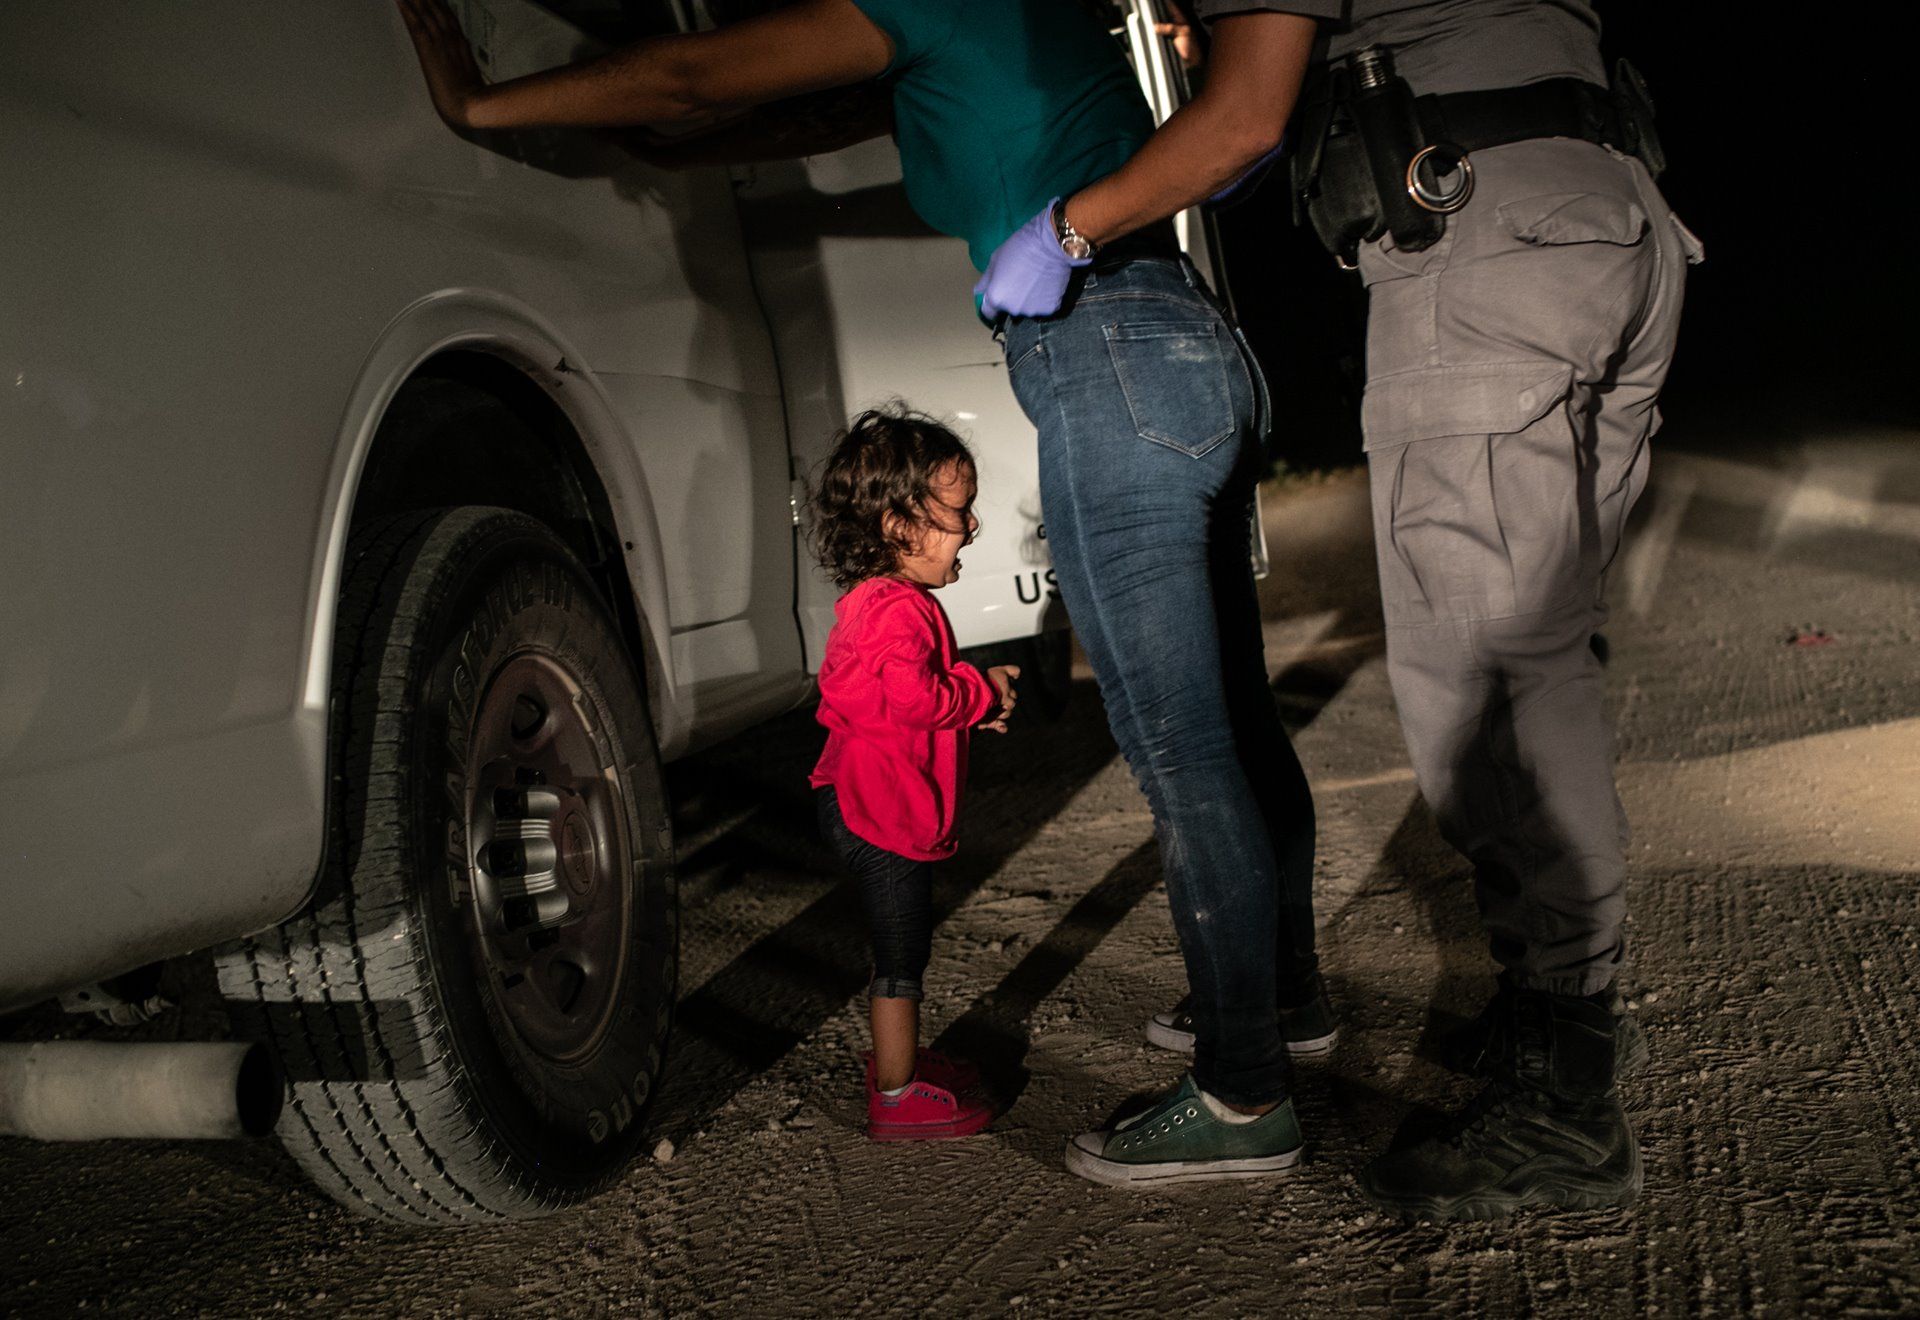
\includegraphics[width=\textwidth,height=\textheight,keepaspectratio]{Images/WPPF-2019PhotoContest-POYNominee-JohnMoore.jpg}
        \caption{\small{\textit{Crying Girl in the Border, John Moore, 18 Junio 2018}}}
        \label{fig:foto}

    \end{figure}
    
    \vspace{0.5cm}

    % TODO: Añadir cita bibliográfica a la imagen 

    \vspace{1cm}
    \hrulefill

\end{titlepage}
\newpage

% NIVEL CONTEXTUAL
En muchas ocasiones demostrar la realidad implica revelar lo que oculta la sociedad detrás de una fachada de irrealidad. 

Esto es lo que quiere mostrar el fotógrafo americano John Moore con esta fotografía realizada en junio de 2018, coincidiendo con la nueva política de Trump relacionada con “cero tolerancia” los inmigrantes, siendo procesados como criminales. 

Mayoritariamente, esto significaba que los niños eran separados de sus padres, siendo la niña de la foto, Yanela Sánchez, también separada de su madre, Sandra Sánchez, siendo llevada a custodia. 

La fotografía se disparó en la frontera de Estados Unidos, más concretamente, en la frontera de McAllen, Texas. 
% TODO: añadir cita bibliográfica

\hrulefill

Podemos definir esta fotografía en el género fotográfico de “prensa” siendo el género más prominente en la fotografía debido a que John Moore es un periodista y fotógrafo para Getty Images. % TODO: Añadir cita a Getty 

También podemos encontrar otros géneros algo más ocultos, ya que en la fotografía contiene un componente social muy marcado, llamando y criticando como se gestionan los inmigrantes en Estados Unidos de formas inhumanas e irrespetuosas. 

Hablando sobre aspectos más técnicos de la imagen, \textit{World Press Photo} nos provee con las características técnicas de la imagen. 
La cámara usada fue una Canon EOS-1D X Mark II % TODO: Conseguir enlace a detalles de cámara 
Una parte muy importante de la fotografía es la sensación de cercanía que otorga la imagen. Se consiguió con objetivo con longitud focal de 35mm.

% NIVEL MORFOLÓGICO

La imagen contiene una gran cantidad de puntualidades que crean una composición bastante cargada, en el que podemos destacar cuatro puntos. 


\end{document}